\documentclass{report}
\usepackage[a4paper, margin=0.5in]{geometry}
\usepackage{parskip}
\usepackage{graphicx}
\usepackage{caption}
\usepackage{amssymb}
\usepackage{amsmath}
\usepackage{algpseudocode}
\usepackage{algorithm}

\captionsetup[figure]{
  font = it,
  labelfont = bf
}

\begin{document}
\begin{minipage}[b]{0.48\textwidth}
    \section*{K-Means Clustering}
    A clustering algorithm is an algorithm designed with the purpose of grouping, into an arbitrary number of classes, a set of points. Such classes are created by to grouping together those points that have common features. Thus, the goal of this category of algorithms is to build knowledge about the data provided as input that makes it possible to find hidden relationships among them which can be used to classify (into one of the classes created in the training stages) a point whose class is not known a priori.
  
    \section*{Standard (or Lloyd) Algorithm}
    In this section, the standard algorithm for implementing k-means clustering is introduced. 
  
    First, it is important to define the initial condition (i.e. the input data) on which the algorithm will be run. Considering the case in two dimensions, the input is a collection of points that are randomly placed in 2D space (Figure \ref{fig:rndpoints}).
  
    \begin{center} 
        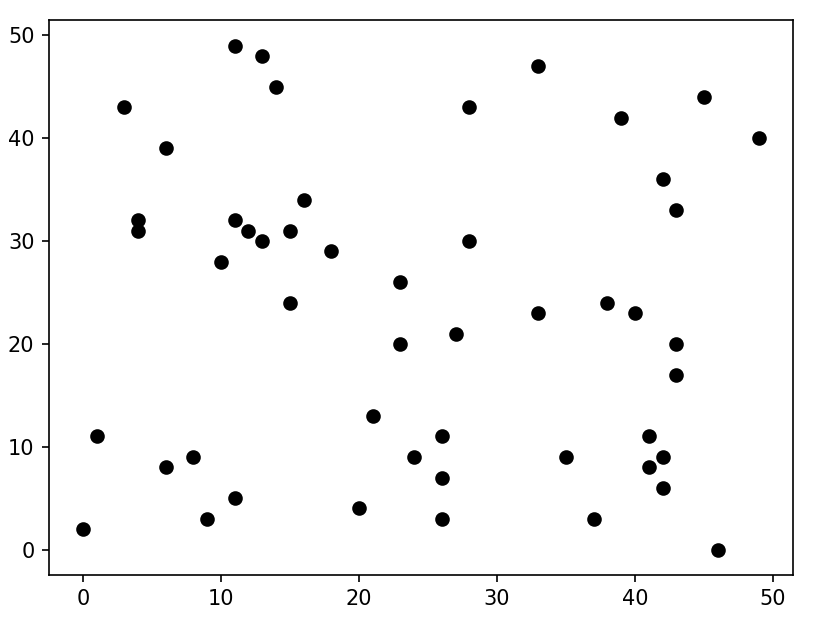
\includegraphics[width = 0.9\textwidth]{imgs/rndpoints.png}
        \captionof{figure}{Initial distribution of random points}
        \label{fig:rndpoints}
    \end{center}
  
    The first step is to generate an arbitrary number of centroids, i.e. points in space representing the classes to which points will be assigned according to a criterion of maximum closeness.
  
    \begin{center}
        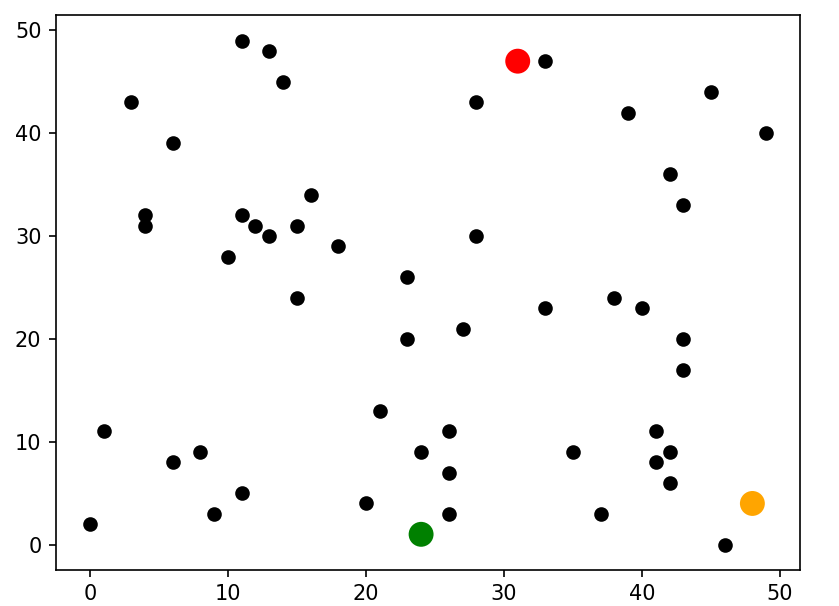
\includegraphics[width = 0.9\textwidth]{imgs/rndcens.png}
        \captionof{figure}{ Random initial position of centroids }
        \label{fig:rndcens}
    \end{center}
  
    Figure \ref{fig:rndcens} shows three centroids representing 3 classes (red, green, orange). The generation of centroids can be done in 2 ways: by choosing some of the points provided as input, or by randomly generating them in space.
  
    After that the centroids are generated, each point is assigned a class according to the principle of maximum closeness. 
\end{minipage}
\hspace{0.1in}
\begin{minipage}[b]{0.48\textwidth}
    Given a point P = (x, y) in space its membership class is the one represented by the centroid whose distance from the point is less than that of all other centroids. The choice of how to measure the distance between two points in space affects the final result of the classification. Therefore it is necessary to specify which measure is being used, in this case the Euclidean distance. Given two points A = ($a_x$, $a_y$) and B = ($b_x$, $b_y$) the Euclidean distance is calculated as
  \begin{equation}
      d(A, B) = \sqrt{(a_x - b_x)^2 + (a_y - b_y)^2}
  \end{equation}

  Figure \ref{fig:pointasgn} shows the points after they have been assigned to the closest centroid.

  \begin{center}    
      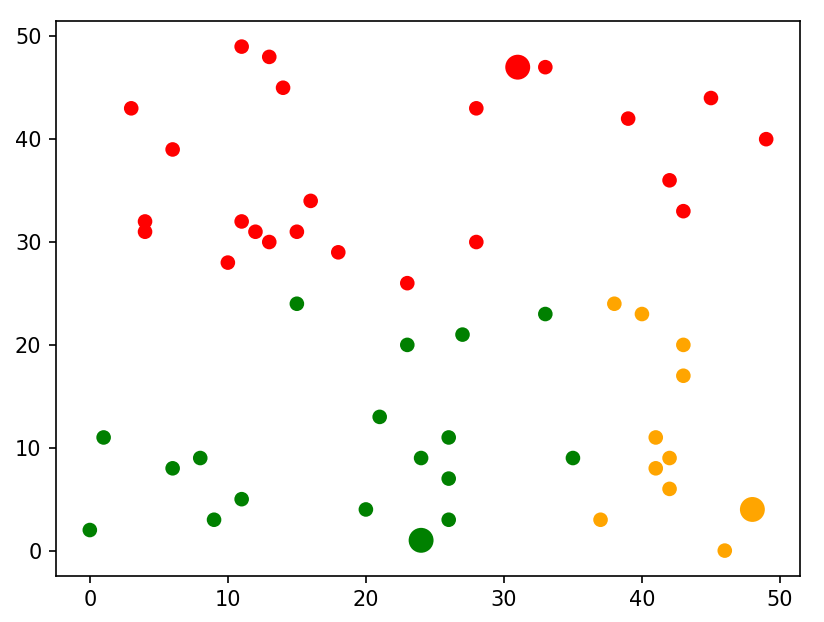
\includegraphics[width = 0.9\textwidth]{imgs/asgnpoints.png}
      \captionof{figure}{Points after the assignation}
      \label{fig:pointasgn}
  \end{center}

  The next step is to reposition the centroids by calculating the average of all points belonging to its class. If $C_i$ is the i-th centroid, its new position ($\tilde{C_i}$) can be calculated as
  \begin{equation}
      \tilde{C_i} = \frac{1}{N_i}\cdot \sum_{p \in C_i} p
      \label{eq:centrep}
  \end{equation}

  Where $N_i$ is the number of points belonging to the i-th class.
  Figure \ref{fig:reccens} shows the centroids after being repositioned. 
  
  \begin{center}    
      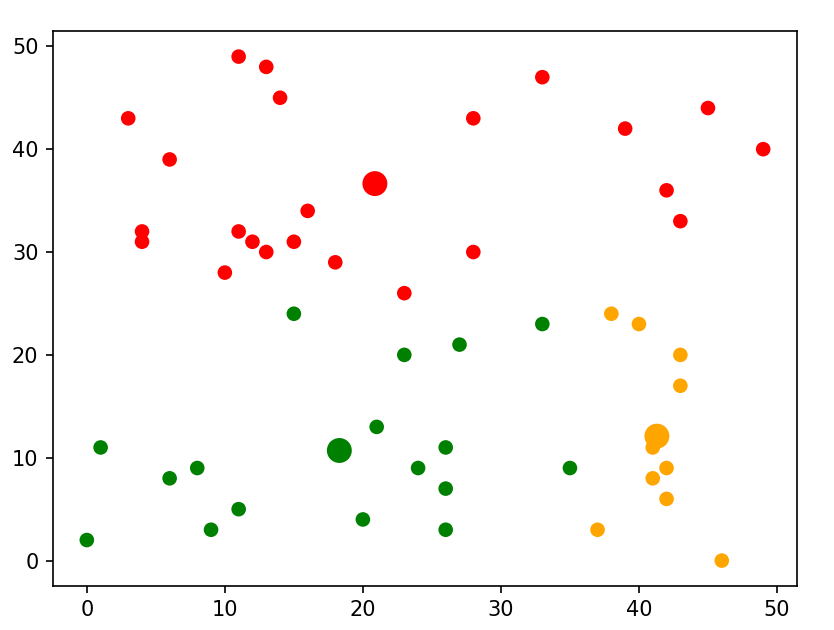
\includegraphics[width = 0.9\textwidth]{imgs/reccens.png}
      \captionof{figure}{Centroids after being recalculated}
      \label{fig:reccens}
  \end{center}

  Now the point assignation is repeated and then the centroid recalculation and so on  until a convergence criterion is reached, which for example could be when the centroids do not shift more than a certain threshold, or simply after a certain number of iterations. This latter method could be usefull when comparing two different algorithm (like lloyd vs hamerly algorithm which is described later)
\end{minipage}

\newpage

\begin{minipage}[b]{0.48\textwidth}
    because the two could converge after a different number of iterations therefore by using a fixed number of repetitions it is easy to compare the result after the same number of cycles. Because of this, for this report, this second approach has been used.

    \section*{Number of iterations}
    The iterations required during a single cycle are \[N\cdot K\cdot d\] where $N$ is the number of points, $K$ is the number of centroids and d is the dimensionality of the data. This is because for each point it is necessary to calculate the distance to each centroid to know which is the least, and to calculate the distance it is necessary to sum k terms (one for each dimension).

    So if m is the number of cycles, the iterations needed are in total
    \begin{equation}
      m(N\cdot K\cdot d)
      \label{eq:lloydcomp}
    \end{equation}

    \begin{algorithm}[H]
        \caption{k-means pseudo-code}\label{alg:cap}
        \begin{algorithmic}
            \State Let "points" be the set of all points
            \State Let "centroids" be the set of all centroids
            \For{ i $<$ iterations }
            \\
            \Comment Point assignation
            \For{ $p$ in points }
                \State mindist = $\min\limits_{j} d(p, C_j)$
                \State old\_centroid = p.centroid\_index
                \State p.centroid\_index = j\\

                \For{l $<$ d}
                    \State coord = p.get\_coord(l)
                    \State average\_per\_class[j][l] += coord

                    \If {old\_centroid $\neq$ -1}
                        \State average\_per\_class[old\_centroid][l] -= coord
                    \EndIf
                \EndFor\\

                \State average\_per\_class[j] += 1
                \If {p.centroid\_index $\neq$ -1}
                    \State average\_per\_class[old\_centroid] -= 1
                \EndIf
            \EndFor
            \\
            \Comment Centroid update

            \For {c in centroids}
                \State nPoints = points\_per\_class[i]
                \For {j $<$ d}
                    \State new\_coord = average\_per\_class[i][j] / nPoints
                    \State c.set\_coord(j, new\_coord)
                \EndFor
            \EndFor
        \EndFor
        \end{algorithmic}
    \end{algorithm}

    \section*{Tracking points belonging to a class}
    During the point assignation step, an important operation is made: tracking which points belong to the classes. In particular we are referring to the following part of the code 
\end{minipage}
\hspace{0.1in}
\begin{minipage}[b]{0.48\textwidth}
    \begin{algorithm}[H]
        \caption{k-means pseudo-code}\label{alg:cap}
        \begin{algorithmic}
            \For{l $<$ d}
                \State coord = p.get\_coord(l)
                \State average\_per\_class[j][l] += coord

                \If {old\_centroid $\neq$ -1}
                    \State average\_per\_class[old\_centroid][l] -= coord
                \EndIf
            \EndFor\\

            \State average\_per\_class[j] += 1
            \If {p.centroid\_index $\neq$ -1}
                \State average\_per\_class[old\_centroid] -= 1
            \EndIf
        \end{algorithmic}
    \end{algorithm}

    Since this is an important process and might not be instantly clear, in this section we will go a little bit deeper and explain how the point tracking is done.

    First of all the average\_per\_class matrix, which is a Kxd matrix that contains, for each row, the sum of all coordinates of the points belonging to that class.

    Then the points\_per\_class array, which is an array with a length of K and, for each class, it contains the number of points which are contained in that class.\\

    Thus, when a point is assigned to the j-th class, its coordinates are added to the average\_per\_class[j] row of the matrix while points\_per\_class[j] is incremented by one.
    It is also important to remove the point from the previous class if it was previously assigned to one. The way to verify it is through the condition $p.centroid\_index != -1$. If the condition is true it means that the points had a previous class. After the verification of the condition, to remove the point from its previous class, its coordinate need to be subtracted from the average\_per\_class[p.centroid\_index] row and points\_per\_class[p.centroid\_index] need to be decremented by one.\\

    Thanks to this process which is done during the points assignation, the following step (i.e. centroid update) is much easier to do. In fact, it is enough to go through the matrix lines and divide it by the total number of points in that class which is contained in the points\_per\_class array.

    \section*{Hamerly's Algorithm}
    Hamerly's algorithm is an optimization of the standard algorithm and expoits the fact that it is not necessary to recalculate the distance of each point from the centroids each time the latter are repositioned. Using the triangular inequality it is, in fact, possible to identify critical points, that is, points for which it is necessary to recalculate the distance to each centroid to find the closest one. In contrast, for the other points, the class to which they were assigned remains the right one even if the centroid has been moved.

    \section*{Triangular inequality}
    Given 3 points A, B, C $\in \mathbb{R}^2$ then  
    \begin{equation}
      |d(A, C) - d(B, C)| \leq d(A, B) \leq d(A, C) + d(B, C)
    \end{equation}

\end{minipage}

\newpage

\begin{minipage}[b]{0.48\textwidth}
    \begin{equation}
        |d(A, B) - d(C, B)| \leq d(A, C) \leq d(A, B) + d(C, B)
        \end{equation}
        \begin{equation}
        |d(C, A) - d(B, A)| \leq d(C, B) \leq d(C, A) + d(B, A)
        \end{equation}
        Where $d(\alpha, \beta)$ is the euclidian distance between the points $\alpha$ and $\beta$. This inequality can also be interpreted geometrically: referring to Figure \ref{fig:triineq}, any side of a triangle is lower than (or equal) to the sum of the other two sides and it is higher (or equal) than the absolute value of the difference between the other two sides.

        \hspace{0.1in}
        \begin{center}
        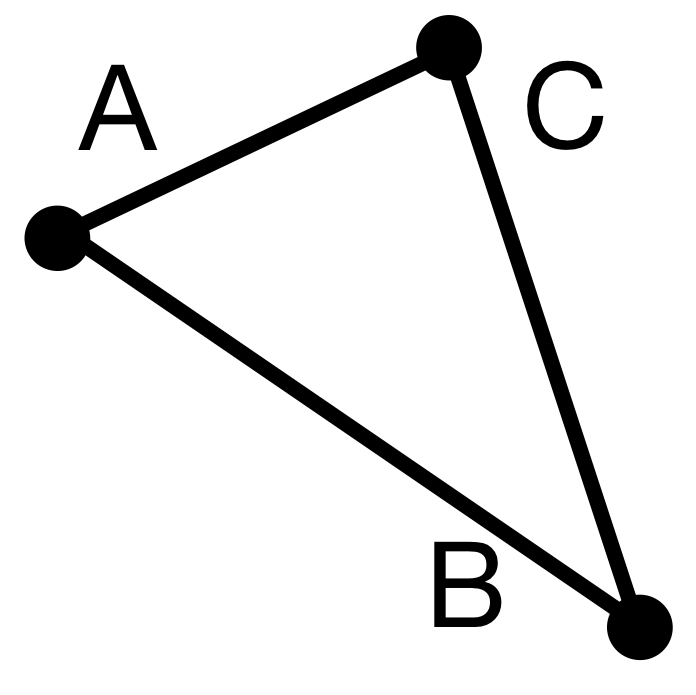
\includegraphics[width = 0.35\textwidth]{imgs/triangle.png}
        \captionof{figure}{3 points in space forming a triangle}
        \label{fig:triineq}
        \end{center}

        \subsubsection*{Triangular inequality and k-means}
        For simplicity, let us assume that we have only one point and two centroids (Figure \ref{fig:triCC}).  

        \begin{center}
            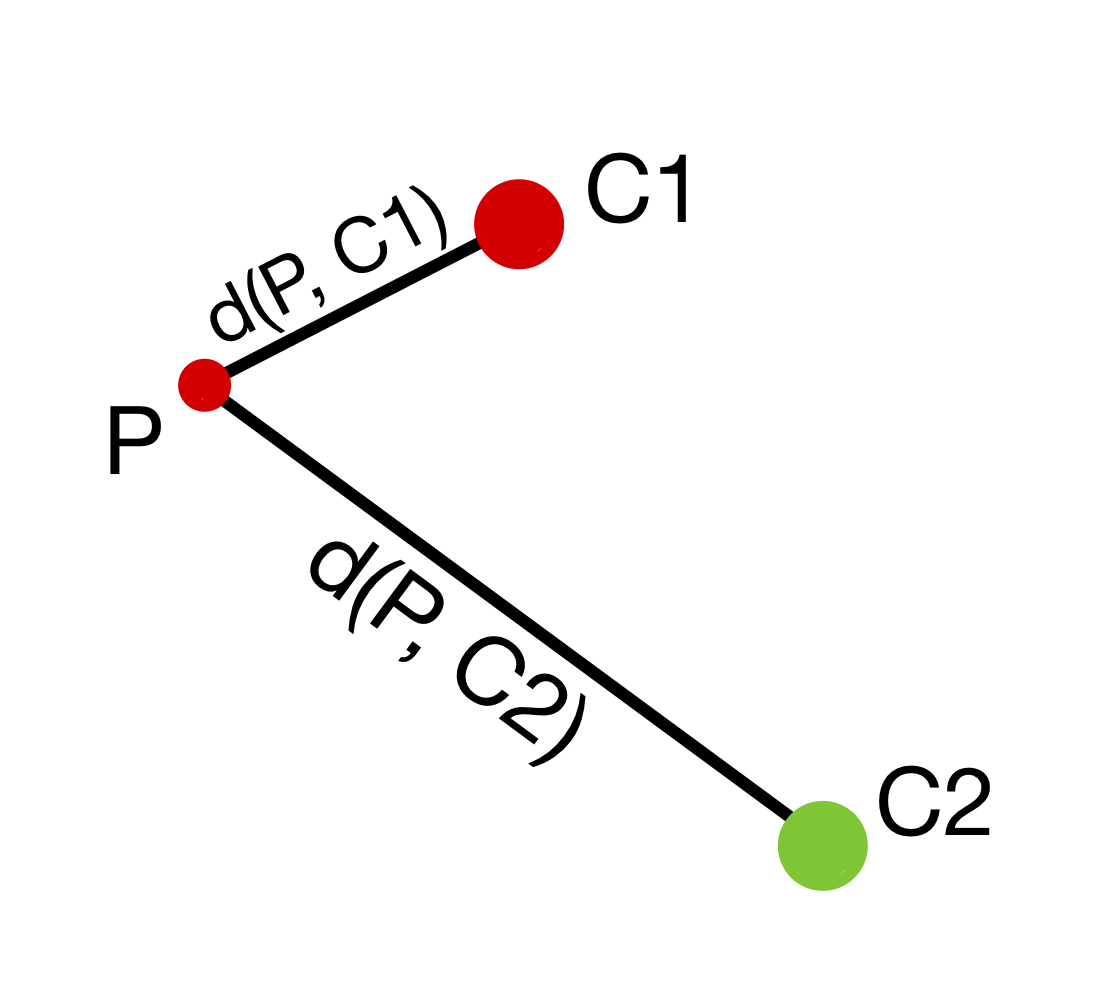
\includegraphics[width = 0.5\textwidth]{imgs/triCC.png}
            \captionof{figure}{Example with 2 centroids and one point}
            \label{fig:triCC}
        \end{center}

        At this point we assume that the centroids shift (Figure \ref{fig:triCCafter}), because of the other points (which are not represented).

        \vspace{0.1in}
        \begin{center}
            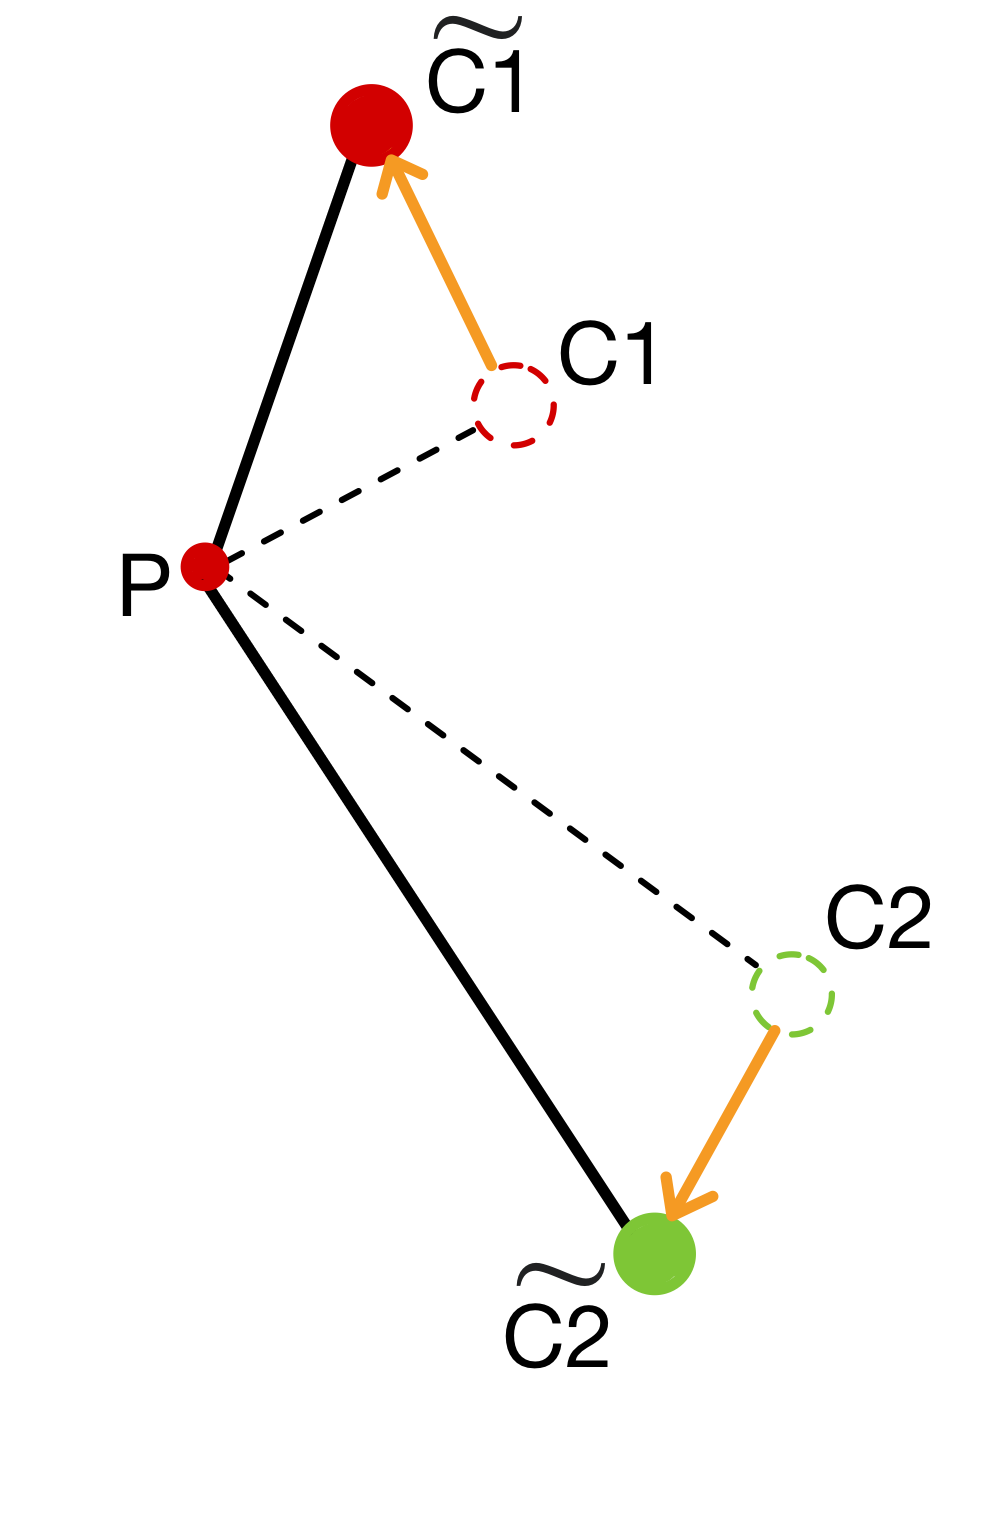
\includegraphics[width = 0.5\textwidth]{imgs/triCCAfter.png}
            \captionof{figure}{Example after the centroids have shifted}
            \label{fig:triCCafter}
        \end{center}   

        Thanks to the triangular inequality, we can state that the distance between P and $\tilde{C_1}$ is:
        \begin{equation*}
          |d(P, C_1) - d(C_1, \tilde{C_1})| \leq d(P, \tilde{C_1}) \leq d(P, C_1) + d(C_1, \tilde{C_1})
        \end{equation*}
        And in the same way:
        \begin{equation*}
          |d(P, C_2) - d(C_2, \tilde{C_2})| \leq d(P, \tilde{C_2}) \leq d(P, C_2) + d(C_2, \tilde{C_2})
        \end{equation*}
\end{minipage}
\hspace{0.1in}
\begin{minipage}[b]{0.48\textwidth}
    Using this result, we can improve the k-means algorithm as follows.
  The first step remains mostly unchanged: it consists of assigning to each point the nearest centroid, and to do this it is necessary to calculate all the distances between the point and the centroids. The difference with the standard algorithm is that in this case, for each point, we will save the distance to the nearest centroid, called upper bound (ub), and also the distance to the second nearest centroid, called lower bound (lb).

  For example, if for a point (P) the nearest centroid is $C_1$ we have that
  \begin{equation}
      ub = d(P, C_1)
  \end{equation}
  \begin{equation}
      lb = \min\limits_{j \neq 1} d(P, C_j)
  \end{equation}

  After the first step, the centroids are repositioned and again the algorithm is almost identical: eqs \ref{eq:centrep} is used to compute the new position of the centroids, but unlike before we will also save the distance traveled by each centroid (using an array with length K called cdistaces), the distance traveled by the centroid that moved the most (maxdist) and its index (maxdist\_index) and the distance traveled by the second centroid that moved the most (secmaxdist).

  At this point, the parameters $ub$ and $lb$ are updated for each point p, as follows.

  \begin{equation}
    ub =  ub + cdistances[p.centroid\_index]
  \end{equation}
  If the closest centroid is also the one that moved the most then
  \begin{equation}
      lb = lb - secmaxdist
  \end{equation}
  Else
  \begin{equation}
      lb = lb - maxdist
  \end{equation}

  These updates are justified by the triangular inequation. In fact, we know that after that the centroids have moved, the point cannot be farther than $ub$ from the nearest centroid and at the same time cannot be closer than $lb$ from the second nearest one.

  Thanks to the previous step, it is possible to identify as critical the points for which $ub \geq lb$, that is, the points for which the assigned centroid may not be the nearest.
  
  The next step is to iterate for all points but recalculating the distance to the nearest centroid only for the critical ones. Moreover, we can optimize this process even more since, once a critical point has been found, it may be sufficient to recalculate only the upper bound, i.e., the distance to the nearest centroid, and then check again the condition $ub \geq lb$ and only if the condition is still verified then it will be necessary to carry out the full calculation of the distances.
  
  Finally, the centroids are updated and the procedure is repeated until the condition of convergence is reached or after a certain number of iterations.

  \section*{Number of iterations}
  In the case of Hamerly's algorithm, the number of iterations required to complete the classification is:
  \begin{equation}
      d\cdot K\cdot N + md(\phi N\cdot K + (1 - \phi)N)
      \label{eq:hamcomp}
  \end{equation}
  Where $\phi$ is the percentage of critical points with respect to the total number of points.
\end{minipage}

\newpage

\begin{minipage}[b]{0.48\textwidth}
    The improvement over the standard algorithm lies in the fact that only the first time it is necessary to compute all the distances, whereas in subsequent iterations, for most points, there is no need to recompute the nearest centroid.

    \section*{Parallelize the Hamerly's algorithm}
  The Hamerly's algorithm has three main sub-tasks: assignation of the points to a class, update of the centroids, update of the lower and upper bounds of all points.

  \subsubsection*{Assignation of the points to a class}
  In this phase, each point will be assigned to a centroid which will represent its class. If it is the first iteration, this can be easly parallelizable by simply partitioning the points between the threads. Each thread will then goes through its set of points and find the minimum distance between the point and the centroids and therefore will assign to point to that class. In this first ieration the work load is equally balanced across the threads because the work that has to be done for each point is the same.

  This is not true from the second iteration, because in this case the only points for which the minimum distance is calculated are the critical points. Therefore it is not enough to partion the points between the threads because criticals points could be not equally distribuited across the point set and because of this some threads could have more work to do compared to others. A load balancing tequiniche has to be used.

  \subsubsection*{Update of the centroids}
  This is the phase where the centroids are moved. Also this step can be easly parallized by simply partitioning the centroids between the threads which, for every of its centroid will compute the new position using the values inside the matrix average\_per\_class and points\_per\_class.

  The work load for every centroid is the same, therefore no special cautions are needed when parallelizing it.

  \subsubsection*{Update the lower and upper bounds of all points}
  During this step, the lower and upper bound of each points are updated using the information saved during the "Update of the centroids" (cdistances, maxdist, maxdist\_index and secmaxdist). This is where the balancing algorithm is applied and the result of this phase is an array (called criticals) containing the address of all critical points that have been found. 

  \subsubsection*{Reduction on the variables average\_per\_class and points\_per\_class}
  When parallelizing the code, a particular cautions has to be taken if two threads wants to add (or subtract) on the same variable.

  This is, in fact, the case for the matrix average\_per\_class and the array points\_per\_class. This is because when calculating the closest class, two threads could find two points that belong to the same class and therefore they both need to update the matrix and increment the array.

  To explain why this is a problem suppose we have a variable v = 42 and two threads that want to modify it as described by the following pseudocode
\end{minipage}
\hspace{0.1in}
\begin{minipage}[b]{0.48\textwidth}
    \begin{algorithm}[H]
        \caption{Parallel update of a variable}
        \begin{algorithmic}
            \If {$thread\_id == 0$}
            \State v = v + 1
            \ElsIf{$thread\_id == 1$}
            \State v = v + 2
            \EndIf
        \end{algorithmic}
    \end{algorithm}

    The expected result is 45 (42 + 1 + 2), however if the code is executed the result might not be 45. This happens if the threads read at the same time the value of v (which is likely to happen in a parallel execution), in that case, they both read 42 and they modify it and then save it back in memory. What happens is that if thread zero is the last to save the value, v would be 43 and, in the same way, if thread one finish later v would be 44.

    The way to solve this problem is called reduction (in this case on the variable v): both thread will have a local memory where they make the changes and when they finish to execute, a sequential algorithm is executed that puts toghether all the changes that have been done.

    OpenMP offer a special clause for that: \#pragma omp parallel reduction(+:v). The first part "\#pragma omp parallel" is just the classic one to start a parallel section, while "reduction(+:v)" is the part that enable reduction. In particular the plus sign specify the operation that will be done by the sequential algorithm on the variable which is specified after the semicolumn. \\
    
    OpenMP also allows to reduce arrays, considering for example the points\_per\_class array, the clause would be: \#pragma omp parallel reduction(+:points\_per\_class[:K]). The same thing is not true for matrices: OpenMP doesn't support matrix reduction. But, it is possible to solve this problem by converting the matrix to an array.

    Let's consider the average\_per\_class $Kxd$ matrix, we can equivalently use an array with a length of $K\cdot d$. In this way we still have the same number of slots for the data and we can access the (i, j) element as by accessing the $(i \cdot d + j)$-th index

    \subsubsection*{Pattern for a parallel access}
    In this section, a general algorithm which has been used a lot in this implementation will be explained: how to partition a set of points between an arbitrary number of threads.

    Suppose that we have N points and T threads, if N was a multiple of T then it would be easy to split the data by using the following algorithm.

    \begin{algorithm}[H]
        \caption{Data partitioning if N mod T = 0}
        \begin{algorithmic}
          \State points\_per\_thread = N / T
          \State ------- Parallel Section -------
          \For{i $<$ points\_per\_thread}
            \State p = points[ points\_per\_thread $\cdot$ thread\_id + i ]
          \EndFor
          \State ----- End Parallel Section -----
        \end{algorithmic}
    \end{algorithm}

    The problem is that N and T are not known a priori and N could not be a multiple of T, therefore we need to properly handle those extra points. First we calculate the points per class and the remainder as
\end{minipage}

\newpage

\begin{minipage}[b]{0.48\textwidth}
    \begin{equation}
        points\_per\_class = Int(\frac{N}{T})
    \end{equation}
    \begin{equation}
        remainder = N\hspace{0.03in}mod\hspace{0.05in} T
    \end{equation}

    Where Int(a) is the integer part of a.
    Thanks to the mod operator properties we know that $remainder < T$. At this point we can assign to the first threads an extra point which can be easly done by checking the thread id as follows:

    \begin{algorithm}[H]
    \caption{Add an extra points to the first threads}
    \begin{algorithmic}
        \State points\_per\_thread = Int(N / T)
        \State remainder = N \% T
        \State ------- Parallel Section -------
        \If {thread\_id $<$ remainder}
        \State points\_per\_class += 1
        \EndIf
        \State ...
        \State ----- End Parallel Section -----
    \end{algorithmic}
    \end{algorithm}

    Also the access pattern needs to be modified because not all threads have the same number of points assigned to them. \\

    The first threads access one more point than the others, therefore they overall introduce a shift equal to the remainder to the points that will be accessed from the last threads. The offset need , therefore, to be added only to the threads accessing a number of points equal to points\_per\_thread (and not points\_per\_thread + 1). The pseudocode then becomes:

    \begin{algorithm}[H]
    \caption{Add an extra points to the first threads}
    \begin{algorithmic}
        \State points\_per\_thread = Int(N / T)
        \State remainder = N \% T
        \State offset = remainder
        \State ------- Parallel Section -------
        \If {thread\_id $<$ remainder}
        \State points\_per\_thread += 1
        \State offset = 0
        \EndIf

        \For {i $<$ points\_per\_thread}
        \State p = points[points\_per\_thread $\cdot$ thread\_id + i + offset]
        \EndFor
        \State ----- End Parallel Section -----
    \end{algorithmic}
    \end{algorithm}
    \section*{Load balancing in standard kMeans}
    Suppose that the standard kMeans algorithm is executed in parallel by splitting between T threads the total points N. In this case the work load is easly divided equally between the threads. In fact we can calculate the total number of points to assign each thread by N/T; if N is not a multiple of T we will also have a reminder
    \begin{equation}
      reminder = N \text{ mod } T < T
    \end{equation}
    If this is the case, we can simply assign the first threads one more point, therefore in the end there will be r threads with N/T + 1 points and T - reminder threads with N/T points.
\end{minipage}
\hspace{0.1in}
\begin{minipage}[b]{0.48\textwidth}
    \section*{Load balancing in Hamerly's algorithm}
    With Hamerly's algorithm, efficient load balancing is not as easy as in the standard version because, for every cycle, it is not neccessary to compute the distances for every points but only for critical ones. Because of this, if the points were simply divided among the threads, it might happen that some have many points while others could have few calculations to do.

    \begin{center}
      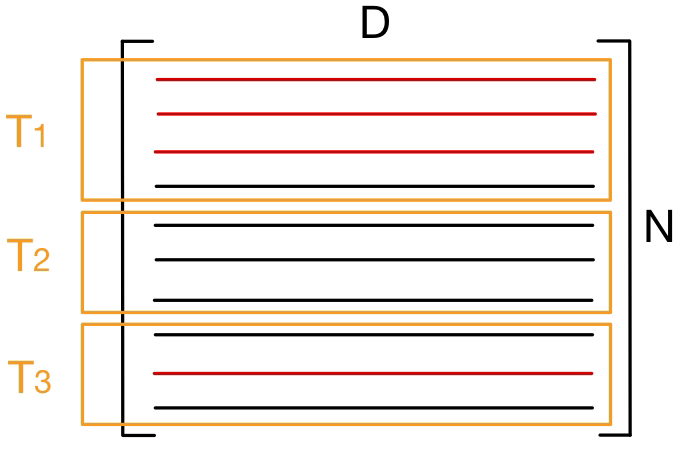
\includegraphics[width = 0.8\textwidth]{imgs/non_balances_hamerly.png}
      \captionof{figure}{Non balanced point division}
      \label{fig:non_bal_ham}
    \end{center}

    The Figure \ref{fig:non_bal_ham} shows an input matrix (N x d, where d is the data dimensionality) where critical points are not  equally distribuited. In this case, the first thread will have three critical points whereas the second thread will have zero.

    To implement an efficient load balacing, a more advanced strategy is needed and one possible solution will be presented in the following part of this report. 
    
    \subsection*{Points assigment for Hamerly's algorithm}
    First of all remember that, in the Hamerly's algorithm, after that each centroid moved it is neccessary to update the upper bound (ub) and the lower bound ($lb$) of each p. This operation can be done in parallel, since the update is indipendent between the points, and the work that has to be done is equal for each p. 

    During this phase, each thread will have a linked list where they add every critical point that it finds, moreover every time it finds a critical it increments by one the value of a global array which has a length of T so that each thread has its own index to access.

    After that all points have been iterated a synchronization is required. During this sequential part it is calculated the total number of critical points (C) that have been found and a second array is created with a length of C.

    At this point, every thread can insert, inside this new array, its critical points. In order to do that, every thread has to start inserting its values from the index which is equal to the sum of the number of criticals found by the previous threads.

    For example, if there are 3 threads and they found respectively [2, 3, 1] criticals then, they start inserting values from the 0, 2 and 5 (2 + 3) index. The objective of this step is to create an array containing all the critical points together because in this way it is possible to equally divide those critical between the threads. 

    If the total number of critical points is $C$ then, the number of criticals to assign each thread can be calculated as $C / T$. If $C$ is not a multiple of T, there will
\end{minipage}

\newpage

\begin{minipage}[b]{0.48\textwidth}
    also be a remainder which can be handled the same way as in the standard case. Below is the pseudo code where N is the total numer of points and "points" is the array containing all points.

    \begin{algorithm}[H]
        \caption{Boundaries update pseudo-code}\label{alg:cap}
        \begin{algorithmic}
          \State --------------------------------------------- \Comment Sequentially
          \State Let nC be the array with the number of criticals found by each thread 
          \State remainder = N \% T
          \State --------------------------------------------- \Comment In Parallel
          \State Let criticals\_per\_thread be the local list of criticals found by the thread
  
          \State$p\_per\_thread = Int(N/T)$
          \State offset = remainder
  
          \If{$thread\_id < remainder$}
            \State $p\_per\_thread = p\_per\_thread + 1$
            \State offset = 0
          \EndIf
  
          \State
          \For{$j < p\_per\_thread$}
            \State p = points[p\_per\_thread $\cdot$ thread\_id + offset + j]
            \State p.ub = p.ub + cdistaces[p.centroid\_index]
            \If{p.centroid\_index == maxdist\_index}
              \State p.lb = p.lb - secmaxdist
            \Else
              \State p.lb = p.lb - maxdist
            \EndIf
  
            \If{p.$ub>$ p.lb}
              \State criticals\_in\_thread.push(p)
              \State nC[thread\_id] = nC[thread\_id] + 1
            \EndIf
          \EndFor
          \State --------------------------------------------- \Comment Sequentially 
          \State C = 0
          \For{j $<$ nC.length}
            \State C = C + nC[j]
          \EndFor
  
          \State Let criticals be the array of all the criticals
          \State --------------------------------------------- \Comment In Parallel 
          \State index = 0
          \For{j $<$ i}
            \State index = index + nC[j]
          \EndFor
          \State 
          \For{j $<$ nC[i]}
            \State criticals[index + j] = criticals\_per\_thread.pop 
          \EndFor
        \end{algorithmic}
    \end{algorithm}

    \subsection*{Insight into the opseudo code}
    Because some of the steps in the pseudocode may not be immediate in understanding what they do and why they are used, this part will give an overview of those instructions that may be less clear.
    \begin{algorithm}[H]
      \caption{$N_i$ increment}
      \begin{algorithmic}
        \If{$thread\_id < remainder$}
          \State $p\_per\_thread = p\_per\_thread + 1$
        \EndIf
      \end{algorithmic}
    \end{algorithm}

    This if statement is implemented to increase by one the number of points that the first threads have to access.
\end{minipage}
\hspace{0.1in}
\raisebox{0in}{
\begin{minipage}[b]{0.48\textwidth}
    \begin{algorithm}[H]
        \caption{p.centroid.distance}
        \begin{algorithmic}
          \State p.ub = p.ub + cdistances[p.centroid\_index]
        \end{algorithmic}
      \end{algorithm}
  
      Through cdistances[p.centroid\_index] we access distance traveled by the centroid to which the point has been assigned.
  
      At every iteration the upper bound of each point, which is accessed by p.ub, has to be updated and the new value will be: p.ub + cdistances[p.centroid\_index]
  
      \begin{algorithm}[H]
        \caption{lower bound update}
        \begin{algorithmic}
          \If{p.centroid\_index == maxdist\_index}
            \State p.lb = p.lb - secmaxdist
          \Else
            \State p.lb = p.lb - maxdist
          \EndIf
        \end{algorithmic}
      \end{algorithm}
  
      When it comes to updating the lower limit, the first thing to check is whether the centroid that moved the most is also the one assigned to the p. In this case, the lower limit cannot be updated with the distance of that centroid because it has already been used for the upper limit, but in this case the distance taken from the second centroid that moved the most has to be used.
  
      \begin{algorithm}[H]
        \caption{lower bound update}
        \begin{algorithmic}
          \State index = 0
          \For{j $<$ thread\_id}
            \State index = index + nC[j]
          \EndFor
        \end{algorithmic}
      \end{algorithm}
  
      This is the part where each thread calculate the index from where it has to start inserting the vales in the global array containing all the critical points.
  
      \begin{algorithm}[H]
        \caption{add values to the global array}
        \begin{algorithmic}
          \For{j $<$ nC[i]}
            \State criticals[index + j] = $L_i$.pop 
          \EndFor       
        \end{algorithmic}
      \end{algorithm}
      This is the last part of the algorithm where every thread inserts into the global array the value of its list.

      \section*{Algorithm testing}
      What has been described up to this point allows to create a parallel kmeans clustering which exploit the Hamerly's algorithm. In this section we present the result of the tests that have been done using the Lloyd, Hamerly and parallelized Hamerly algorithm to compare the performances.

      \subsubsection*{2D random dataset}
      The first dataset on which the tests were run is a two dimensional, randomly generated, dataset containing 50000. In addition, 3 centroids have been also randomly generated. 

      The test starts by picking the first 500 points in the dataset and run the clustering on them to measure the time the algorithm takes,
\end{minipage}}

\newpage

\begin{minipage}[b]{0.48\textwidth}
  then the process is repeated by increasing the number of point by 500 points per iterations up to when the total number of points is used. Every time the number of points increases the time taken for the execution is measured such that it is possible to plot a time versus number of points graph.

  This process has been done for the aforementioned algorithms to produce the following graph
  
  \begin{center} 
    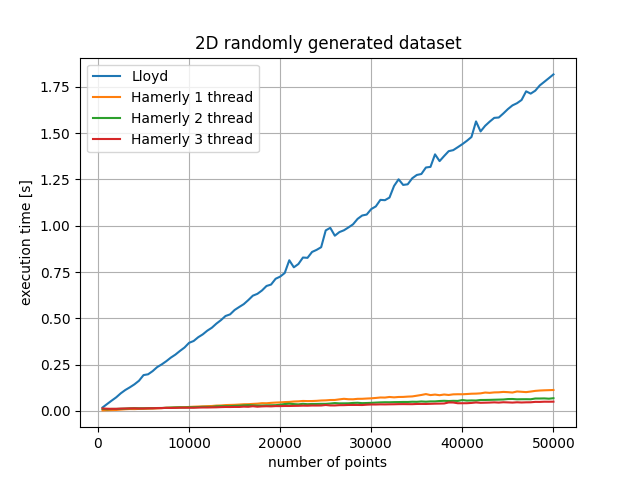
\includegraphics[width = 1\textwidth]{imgs/lh123_2Drnd.png}
    \captionof{figure}{result of the test on the 2D randomly generated dataset}
    \label{fig:lh123_2Drnd}
  \end{center}

  First of all notice that, for all the algorithm, the plot is a straight line. This is as expected if we consider the time complexity of both Lloyd and Hamerly algorithm eq. \ref{eq:lloydcomp} and \ref{eq:hamcomp}, in both cases it is possible to factor the number of points (N) out to obtain an eqation of the type mN.\\

  Talking about the performance, the hamerly algorithm even with 1 thread shows a remarkable speedup with respect to the Lloyd algorithm. Considering the case with 50000 points, the Lloyd algorithm takes 1.81738 seconds while the hamerly algorithm with 1 thread takes 0.113175 seconds, which is approximately 93\% faster. 
  
  By increasing the number of threads, the plot shows an additional speedup: with 2 threads (0.0686808s) the speedup, with respect to the 1 thread hamerly algorithm (0.113175s), is approximately 40\%. As expected, the time taken with 2 threads is not twice the time with 1 thread because some part of the code still be executed sequentially.

  Lastly, the time taken with 3 threads is 0.0500831 which result in an addition 27\% speedup. We can clearly see that by increasing the number of threads the speedup tends to get smaller, this is as expected and can be proven mathematically. Assuming an ideal speedup, i.e. the time taken by T threads is $\frac{t_1}{T}$ where $t_1$ is the time taken by 1 thread, the time difference between 2 consecutive number of threads can be expressed as
  \begin{equation*}
    \Delta t = t_1 ( \frac{1}{T} - \frac{1}{T + 1} )
  \end{equation*}
  If T tends to infinity $\Delta t$ tends to zero.

  \subsubsection*{3D random dataset}
  To test with a different dataset, the second one used is a three dimension randomly generated dataset (always with 50000 points and 3 centoids).

  The used procedure remains the same used also before,
\end{minipage}
\hspace{0.1in}
\begin{minipage}[b]{0.48\textwidth}
  i.e. starting  with a low number of points and increase them gradually (500 points per iteration) to plot the time versus number of points graph.

  \begin{center} 
    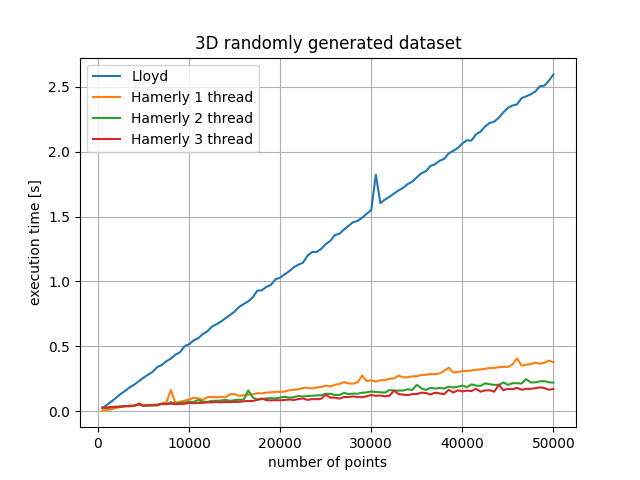
\includegraphics[width = 0.9\textwidth]{imgs/lh123_3Drnd.png}
    \captionof{figure}{result of the test on the 3D randomly generated dataset}
    \label{fig:lh123_3Drnd}
  \end{center}

  The previous pattern can be seen also in this plot: the lloyd algorithm is considerably slower than the hamerly algorithm with 1 thread and then an additional speedup is obtained by increasing the number of threads.

  By considering the case with 50000 points the time taken by the different algorithms are 2.59356 second for Lloyd, 0.378505 seconds for Hamerly with 1 thread, 0.221699 seconds for Hamerly with 2 threads and 0.173437 seconds.

  The speedup between two consecutive "lines" are respectively: 86\% (lloyd vs hamerly 1 thread), 42\% (hamerly 1 thread vs 2 threads), 22\% (hamerly 2 threads vs 3 threads). Again we notice that as the threads increase the speedup decreases.

  \subsubsection*{Wine quality dataset}
  To test the algorithm with a more realisitc dataset, we downloaded a dataset which contains features about different wines which can be used to group them in classes representing their quality between 0 and 10.

  The number of points in the dataset is 1143, with a dimensionality of 11. The centroids are 10 and were generated by randomly select 10 points between the whole dataset.\\

  Other than that, the procedure remains the same but this time the step taken at each iteration to increase the number of points is 9. The result of this test is reported in the followiing graph

  \begin{center} 
    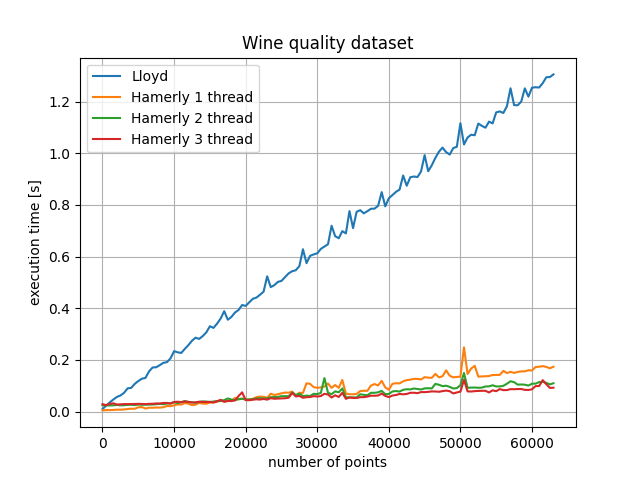
\includegraphics[width = 0.9\textwidth]{imgs/lh123_wine.png}
    \captionof{figure}{result of the test on wine dataset}
    \label{fig:lh123_wine}
  \end{center}
\end{minipage}

\newpage

\begin{minipage}[b]{0.48\textwidth}
  By considering the case with 50000 points the time taken by the different algorithms are 1.30501 second for Lloyd, 0.173809 seconds for Hamerly with 1 thread, 0.109867 seconds for Hamerly with 2 threads and 0.0925767 seconds.

  The speedup between two consecutive "lines" are respectively: 87\% (lloyd vs hamerly 1 thread), 34\% (hamerly 1 thread vs 2 threads), 16\% (hamerly 2 threads vs 3 threads).
\end{minipage}
\hspace{0.1in}
\begin{minipage}[b]{0.48\textwidth}
\end{minipage}

\end{document}